\documentclass[12pt, twoside]{article}
\usepackage[letterpaper, margin=1in, headsep=0.5in]{geometry}
\usepackage[english]{babel}
\usepackage[utf8]{inputenc}
\usepackage{amsmath}
\usepackage{amsfonts}
\usepackage{amssymb}
\usepackage{tikz}
\usetikzlibrary{quotes, angles}
\usepackage{graphicx}
\usepackage{enumitem}
\usepackage{multicol}

\newif\ifmeta
\metatrue %print standards and topics tags

\title{Regents Geometry}
\author{Chris Huson}
\date{December 2021}

\usepackage{fancyhdr}
\pagestyle{fancy}
\fancyhf{}
\renewcommand{\headrulewidth}{0pt} % disable the underline of the header
\raggedbottom


\fancyhead[LE]{\thepage}
\fancyhead[RO]{\thepage \\ Name: \hspace{4cm} \,\\}
\fancyhead[LO]{BECA / Dr. Huson / Geometry 5 Congruence Transformations}

\begin{document}

\subsubsection*{5.3 Classwork: Rotation \hfill CCSS.HSG.CO.A.5}
\begin{enumerate}
  \item Do Now: Reflect $\triangle JKL$ across the $y$-axis, labeling the image $\triangle J'K'L'$.
  \begin{center}
      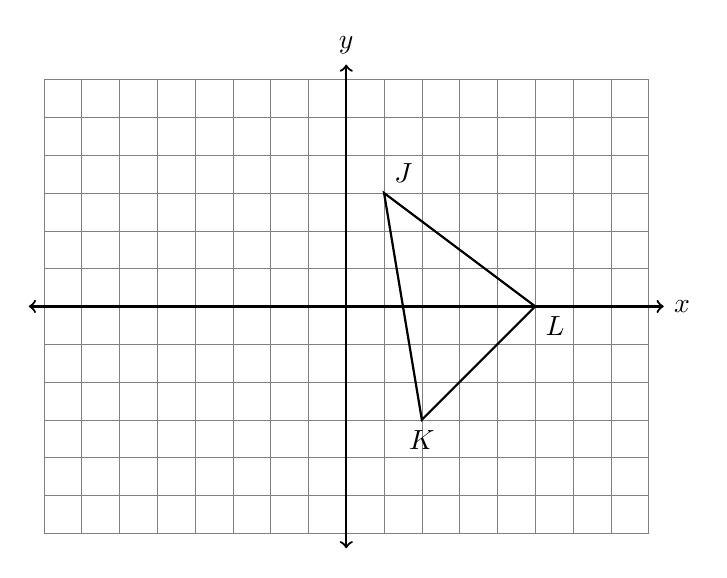
\begin{tikzpicture}[scale=.48]
      \draw [help lines] (-8,-6) grid (8,6);
      \draw [thick, <->] (-8.4,0) -- (8.4,0) node [right] {$x$};
      \draw [thick, <->] (0,-6.4)--(0,6.4) node [above] {$y$};  
      \draw [thick]
        (1,3) node[above right] {$J$}--
        (2,-3) node[below] {$K$}--
        (5,0) node[below right] {$L$}--cycle;  
    \end{tikzpicture}
  \end{center}
  
  \item On the axes below, mark and label the origin, $O(0,0)$. Plot the point $P(4,1)$ and segment $\overline{OP}$. Graph its image, $\overline{O'P'}$, after a $90^\circ$ counterclockwise rotation around the origin. Mark $P'$ and write it down as a coordinate pair.
    \begin{center}
      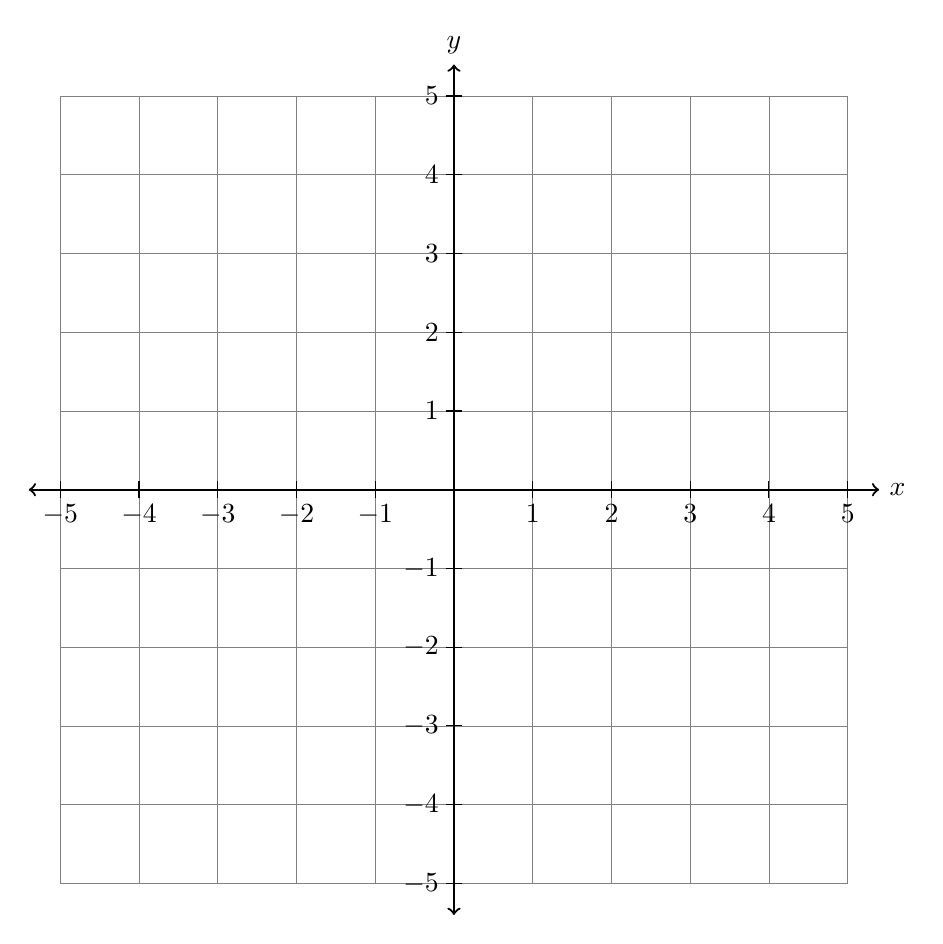
\begin{tikzpicture}[scale=1]
      \draw [help lines] (-5,-5) grid (5,5);
      \draw [thick, <->] (-5.4,0) -- (5.4,0) node [right] {$x$};
      \draw [thick, <->] (0,-5.4)--(0,5.4) node [above] {$y$};
      \foreach \x in {-5,...,-1,1,2,3,4,5}
        \draw[shift={(\x,0)},color=black] (0pt,-3pt) -- (0pt,3pt) node[below=5pt]  {$\x$};
      \foreach \y in {-5,...,-1,1,2,3,4,5}
        \draw[shift={(0,\y)},color=black] (-3pt,0pt) -- (3pt,0pt) node[left=5pt]  {$\y$}; 
    \end{tikzpicture}
  \end{center}

\newpage
\item A rotation maps triangle $DEF$ onto triangle $LMN$. \\[0.5cm]
Write the letter or letters for each corresponding object. \vspace{0.5cm}
    \begin{multicols}{2}
      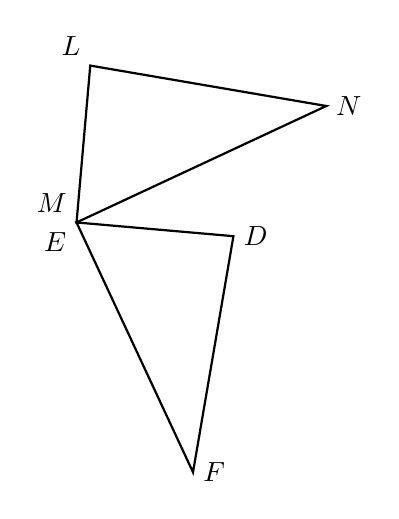
\begin{tikzpicture}[scale=1]
        \coordinate [label=above left:$L$](A) at (85:2);
        \coordinate [label=above left:$M$](B) at (0, 0);
        \coordinate [label=right:$N$](C) at (25:3.5);
        \draw [thick] (A)--(B)--(C)--cycle;
        \draw [thick, rotate=-90] (85:2) node[right]{$D$}--
        (0,0) node[below left]{$E$}--
        (25:3.5) node[right]{$F$}--cycle;
      \end{tikzpicture}

      \begin{enumerate}
        \item $E \rightarrow$ \vspace{1.5cm}
        \item $F \rightarrow$ \vspace{1.5cm}
        \item $\overline{DF} \rightarrow$ \vspace{1.5cm}
      \end{enumerate}
    \end{multicols}

\item A rotation centered at the origin maps $A$ to $A'$, as shown, $A(3,1) \rightarrow A'(-1,3)$.
\begin{multicols}{2}
  \begin{enumerate}
    \item Which correctly identifies the rotation?
    \begin{enumerate}[label=(\Alph*)]
      \item Clockwise $180^\circ$
      \item Counter clockwise $180^\circ$
      \item Clockwise $90^\circ$
      \item Counter clockwise $90^\circ$
      \item None of the above
    \end{enumerate} \vspace{2cm}
    %\item What is the horizontal shift, how many squares right or left? \vspace{1.25cm}
    %\item What is the vertical shift, how many squares up or down? \vspace{1.25cm}
    \item If the same translation is applied to $C(5,1)\rightarrow C'(x,y)$, plot and label the point $C'$ as an ordered pair.
    \end{enumerate}
    \begin{flushright}
    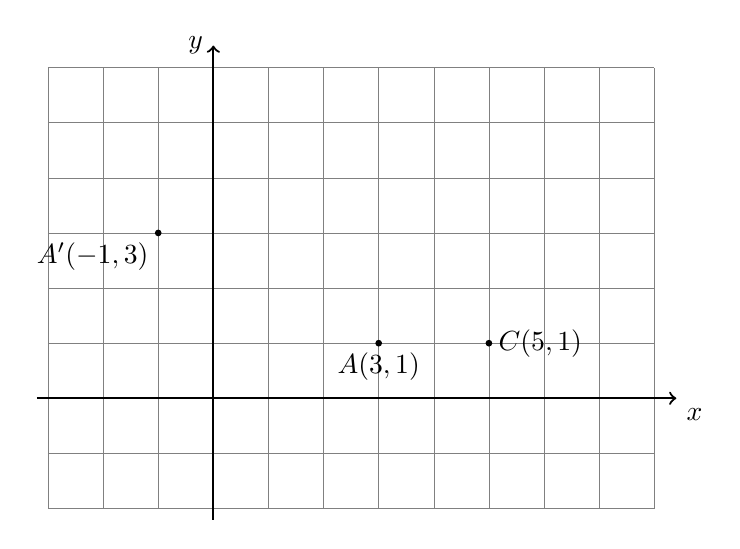
\begin{tikzpicture}[scale=0.7]
      \draw [help lines] (-3,-2) grid (8,6);
      \draw [thick, ->] (-3.2,0) -- (8.4,0) node [below right] {$x$};
      \draw [thick, ->] (0,-2.2)--(0,6.4) node [left] {$y$};
      \draw [fill] (3,1) circle [radius=0.05] node[below] {$A(3,1)$};
      \draw [fill] (-1,3) circle [radius=0.05] node[below left] {$A'(-1,3)$};
      %\draw [->, dashed] (7,1)--(2,3);
      \draw [fill] (5,1) circle [radius=0.05] node[right] {$C(5,1)$};
    \end{tikzpicture}
    \end{flushright}
\end{multicols}

\newpage
\item Rotate the triangle $90^\circ$ clockwise around the origin, $\triangle ABC \rightarrow \triangle A'B'C'$. Complete the table of the coordinates and plot and label the image on the grid. \vspace{0.5cm}
\begin{multicols}{2}
  $A(1,2) \rightarrow$ \\[0.7cm]
  $B(1,4) \rightarrow$ \\[0.7cm]
  $C(4,2) \rightarrow$ \\[0.7cm]
    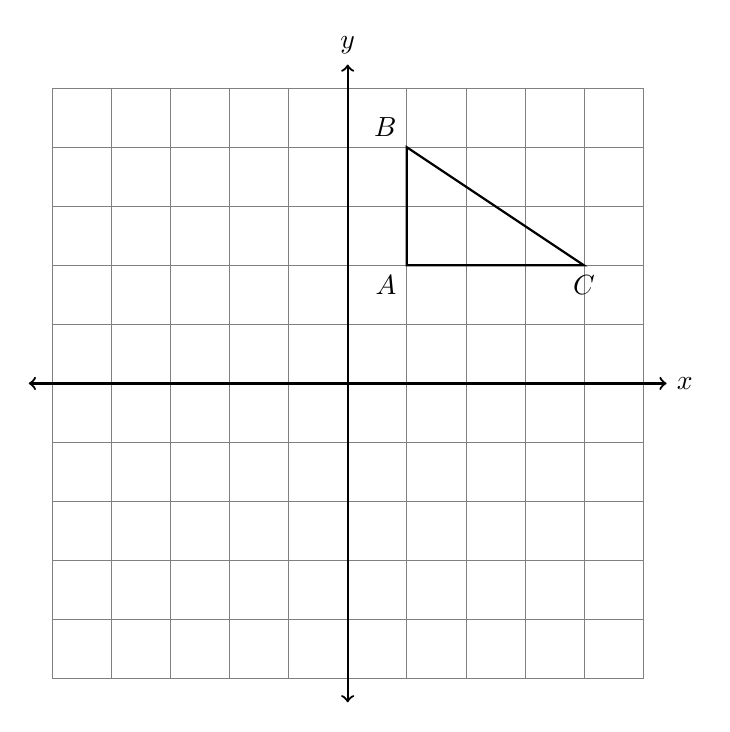
\begin{tikzpicture}[scale=.75]
    \draw [help lines] (-5,-5) grid (5,5);
    \draw [thick, <->] (-5.4,0) -- (5.4,0) node [right] {$x$};
    \draw [thick, <->] (0,-5.4)--(0,5.4) node [above] {$y$};  
    \draw [thick]
      (1,2) node[below left] {$A$}--
      (1,4) node[above left] {$B$}--
      (4,2) node[below] {$C$}--cycle;  
    \end{tikzpicture}
  \end{multicols}

\item $\triangle ABC$ is shown with vertices $A(-1,2)$, $B(6,1)$, and $C(5,4)$. Rotate the triangle $90^\circ$ counter clockwise around the origin. Write down its coordinates in a table and plot and label it on the graph.
  \begin{flushright}
    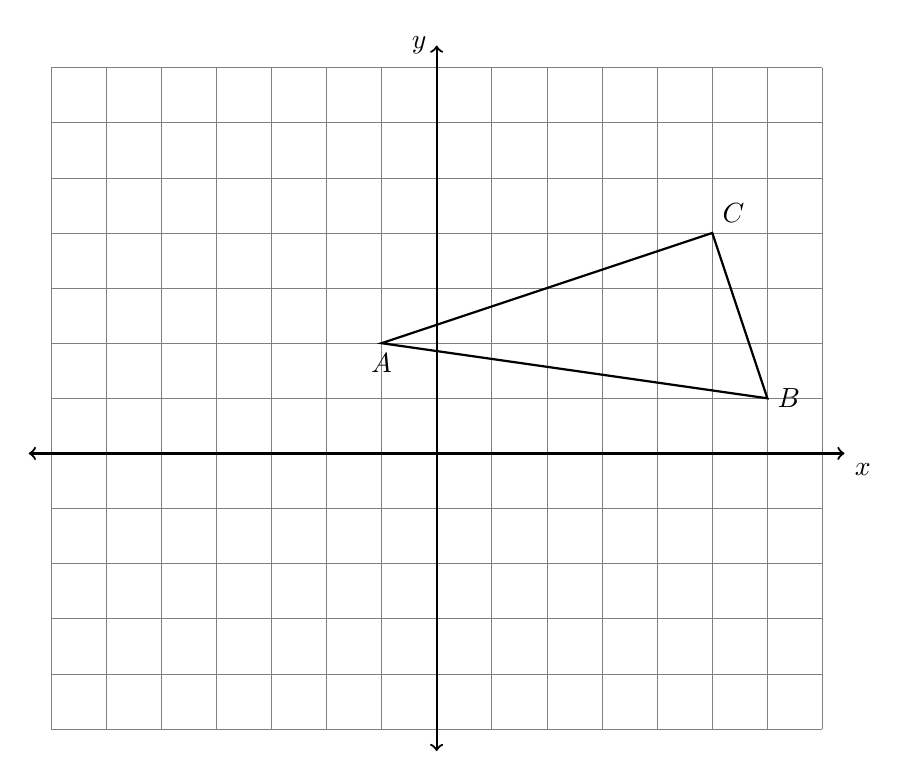
\begin{tikzpicture}[scale=0.7]
      \draw [help lines] (-7,-5) grid (7,7);
      \draw [thick, <->] (-7.4,0) -- (7.4,0) node [below right] {$x$};
      \draw [thick, <->] (0,-5.4)--(0,7.4) node [left] {$y$};
      \draw [thick] (-1,2) node[below] {$A$}--
        (6,1) node[right] {$B$}--
        (5,4) node[above right] {$C$}--
        cycle;
    \end{tikzpicture}
    \end{flushright}

\newpage
  \item Given $\triangle WIN \cong \triangle W'I'N'$. Describe the rigid motion mapping $\triangle WIN \rightarrow \triangle W'I'N'$.
  \begin{flushright}
    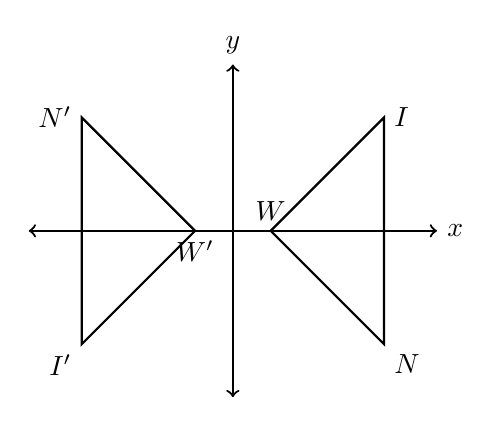
\begin{tikzpicture}[scale=.48]
      %\draw [help lines] (-10,-7) grid (10,7);
      \draw [thick, <->] (-5.4,0) -- (5.4,0) node [right] {$x$};
      \draw [thick, <->] (0,-4.4)--(0,4.4) node [above] {$y$};  
      \draw [thick]
      (1,0) node[above] {$W$}--
      (4,3) node[right] {$I$}--
      (4,-3) node[below right] {$N$}--cycle;
      \draw [thick]
      (-1,0) node[below] {$W'$}--
      (-4,3) node[left] {$N'$}--
      (-4,-3) node[below left] {$I'$}--cycle;
    \end{tikzpicture}
  \end{flushright}

  \item Determine and state the sequence of transformations applied to map $BECA$ to $B''E''C''A''$.
  \begin{flushright}
      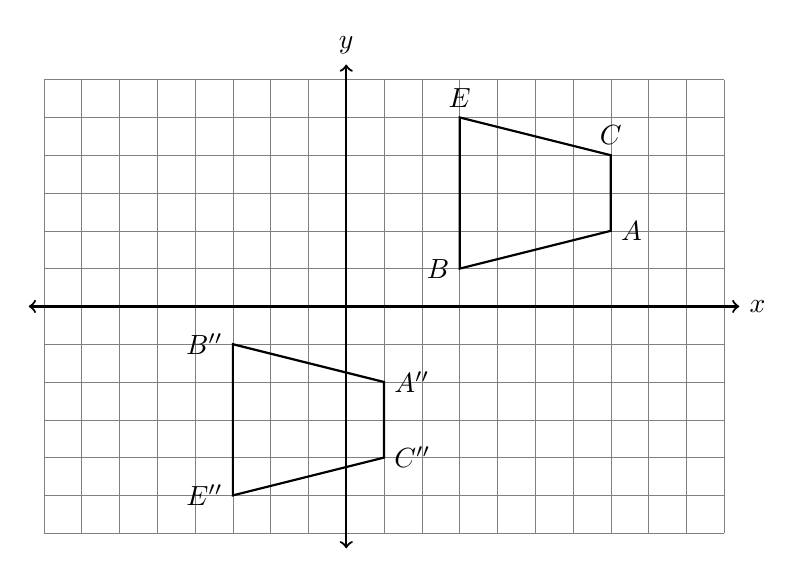
\begin{tikzpicture}[scale=.48]
      \draw [help lines] (-8,-6) grid (10,6);
      \draw [thick, <->] (-8.4,0) -- (10.4,0) node [right] {$x$};
      \draw [thick, <->] (0,-6.4)--(0,6.4) node [above] {$y$};  
      \draw [thick]
        (3,1) node[left] {$B$}--
        (3,5) node[above] {$E$}--
        (7,4) node[above] {$C$}--
        (7,2) node[right] {$A$}--cycle;
      \draw [thick]
        (-3,-1) node[left] {$B''$}--
        (-3,-5) node[left] {$E''$}--
        (1,-4) node[right] {$C''$}--
        (1,-2) node[right] {$A''$}--cycle; 
    \end{tikzpicture}
  \end{flushright}

  \item Determine and state the transformation mapping $\triangle NOP$ onto $\triangle QRP$. 
    \begin{flushright}
        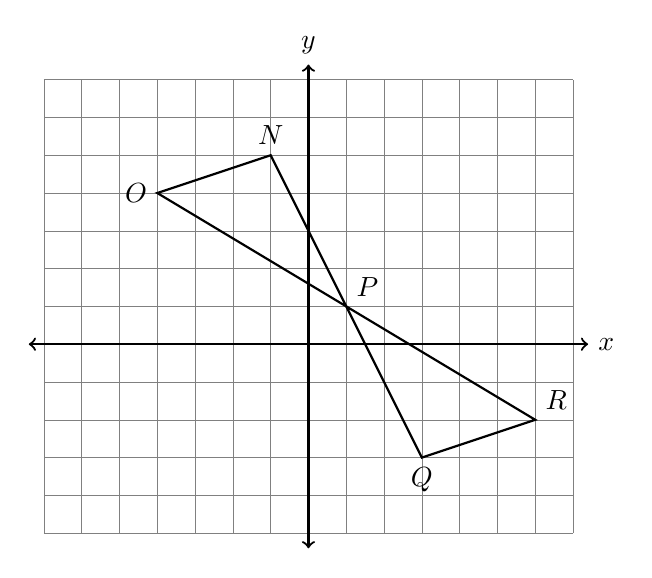
\begin{tikzpicture}[scale=.48]
        \draw [help lines] (-7,-5) grid (7,7);
        \draw [thick, <->] (-7.4,0) -- (7.4,0) node [right] {$x$};
        \draw [thick, <->] (0,-5.4)--(0,7.4) node [above] {$y$};  
        \draw [thick]
          (-1,5) node[above] {$N$}--
          (-4,4) node[left] {$O$}--
          (1,1) --cycle;
        \draw [thick]
        (3,-3) node[below] {$Q$}--
        (6,-2) node[above right] {$R$}--
        (1,1) node[above right] {$P$}--cycle;
      \end{tikzpicture}
    \end{flushright}

\end{enumerate}
\end{document}

\newpage
  \item The quadrilateral $ROCK$ undergoes rigid motions, shown below. Describe the sequence of transformations applied.
  \begin{flushright}
      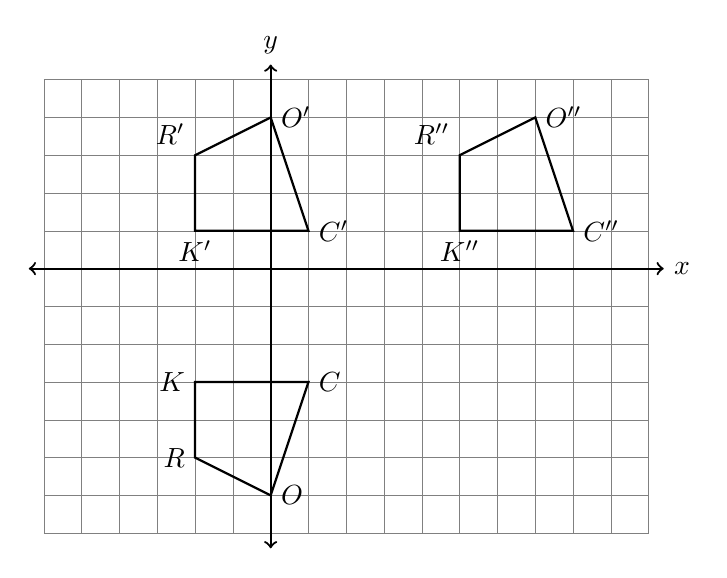
\begin{tikzpicture}[scale=.48]
      \draw [help lines] (-6,-7) grid (10,5);
      \draw [thick, <->] (-6.4,0) -- (10.4,0) node [right] {$x$};
      \draw [thick, <->] (0,-7.4)--(0,5.4) node [above] {$y$};  
      \draw [thick]
        (5,1) node[below] {$K''$}--
        (5,3) node[above left] {$R''$}--
        (7,4) node[right] {$O''$}--
        (8,1) node[right] {$C''$}--cycle;
      \draw [thick]
        (-2,1) node[below] {$K'$}--
        (-2,3) node[above left] {$R'$}--
        (0,4) node[right] {$O'$}--
        (1,1) node[right] {$C'$}--cycle;  
      \draw [thick]
      (-2,-3) node[left] {$K$}--
      (-2,-5) node[left] {$R$}--
      (0,-6) node[right] {$O$}--
      (1,-3) node[right] {$C$}--cycle;
    \end{tikzpicture}
  \end{flushright}

  \item The quadrilateral $MATH$ is mapped to $M'A'T'H'$ by a rigid motion. What transformation a been applied?  \vspace{0.5cm}
  \begin{multicols}{2}
    \begin{enumerate}
      \item Dilation
      \item Reflection
      \item Rotation
      \item Translation
    \end{enumerate}
    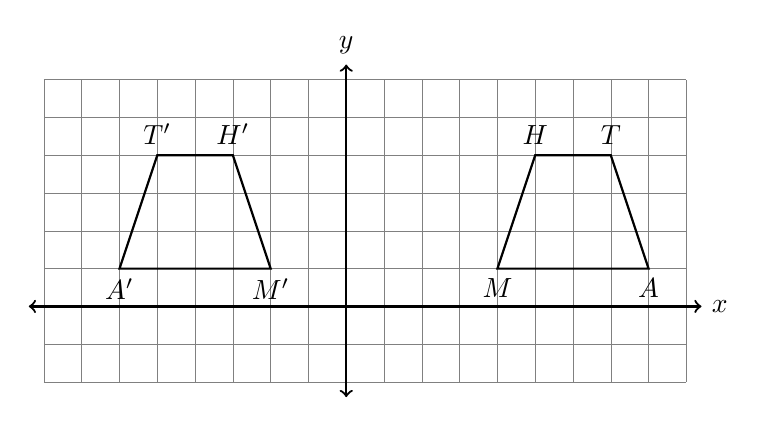
\begin{tikzpicture}[scale=.48]
      \draw [help lines] (-8,-2) grid (9,6);
      \draw [thick, <->] (-8.4,0) -- (9.4,0) node [right] {$x$};
      \draw [thick, <->] (0,-2.4)--(0,6.4) node [above] {$y$};  
      \draw [thick]
        (4,1) node[below] {$M$}--
        (8,1) node[below] {$A$}--
        (7,4) node[above] {$T$}--
        (5,4) node[above] {$H$}--cycle;
      \draw [thick]
        (-2,1) node[below] {$M'$}--
        (-6,1) node[below] {$A'$}--
        (-5,4) node[above] {$T'$}--
        (-3,4) node[above] {$H'$}--cycle; 
    \end{tikzpicture}
  \end{multicols}